% !TEX program = xelatex
% !TEX options = --shell-escape -synctex=1 -interaction=nonstopmode -file-line-error "%DOC%"
\documentclass{ctexart}
\usepackage{hyperref}
\usepackage{url}
\usepackage{multirow}
\usepackage{multicol}
\usepackage{float}
\usepackage{verbatim}
\usepackage{authblk}
\usepackage{amsmath}
\usepackage{amsfonts}
\usepackage{amssymb}
\usepackage{mathrsfs}
\usepackage{bm}
\usepackage{pdfpages}

\title{$\alpha$与$\beta$粒子鉴别程序设计报告}
\author[1]{徐大成}
\author[2]{武益阳}
\affil[1]{清华大学工程物理系}
\affil[2]{清华大学物理系}
\date{2020年5月}

\begin{document}

\maketitle

\newpage
\tableofcontents

\begin{abstract}
    本报告设计了一个卷积神经网络(Convolutional Neural Network, CNN),来处理Jinping中微子实验1吨原型机上的$\alpha$与$\beta$粒子鉴别问题。
    算法以1吨原型机上的30个光电倍增管(Photomultiplier Tube, PMT)的输出电压为输入数据,直接输出CNN对$\alpha$与$\beta$两种粒子的预测概率。
    使用ROC曲线(Receiver Operating Characteristic Curve)来对算法输出结果进行判别,AUC(Area Under the Curve of ROC)可以达到最高0.752。
\end{abstract}

\textit{关键词}:卷积神经网络、粒子鉴别、ROC

\section{问题背景}
中微子是已知的基本粒子之一,只参与弱相互作用,与物质相互作用的散射截面极小。对中微子的质量及CP对称破缺等性质的研究,会揭示超越现有模型的物理规律。
在中微子实验装置中,不可避免地会存在一些本底放射源,对这些放射源的种类及浓度等研究是中微子实验的基础。
Jinping中微子实验中,放射源释放的$\alpha$与$\beta$粒子会引起液闪发光,我们可以通过分析这些光子的信息来对$\alpha$与$\beta$粒子进行鉴别。
光电倍增管(Photomultiplier Tube, PMT)作为灵敏的单光子探测器,被广泛应用于大型液体中微子实验探测装置中,是当今唯一无法替代的电子管设备。
在Jinping中微子实验中,PMT会接收到$\alpha$与$\beta$粒子在液闪中产生的光信号。

\section{方法回顾}
\subsection{闪烁光时间尺度法}
通过对模拟数据的分析及前人对液体闪烁体的性质研究,可以知道$\alpha$粒子的长寿命激发较多,液闪发光时间的尺度较大。
据此,可以分析每个事件中光子击中PMT的时间分布的标准差,建立此标准差与概率之间的线性映射关系($\sigma \in \mathbb{R}^{+} \rightarrow (0,1)$),
映射关系形如:($x = \sigma$)

$y = \begin{cases}
    0 & x \leq t_{1} \\
    \frac{1}{t_{2}-t_{1}}x-\frac{t_{1}}{t_{2}-t_{1}} & t_{1} < x \leq t_{2} \\
    1 & x > t_{2} \\
\end{cases}$

其中$t_{1},t_{2}$可以由遍历或交叉验证(Cross Validation)确定。

\subsection{切伦科夫环识别法}
$\beta$粒子本质为电子,质量远小于$\alpha$粒子。相同能量的$\beta$粒子比$\alpha$粒子速度快。
当$\beta$粒子的速度超过液闪中的光速时,$\beta$粒子的运动会产生切伦科夫光(Cherenkov radiation),在PMT阵列上会产生切伦科夫环图样。
可以通过对切伦科夫环的识别来鉴别$\alpha$与$\beta$粒子。

\section{算法}
我们随后设计了一个卷积神经网络,以30个PMT在1029ns的采样时间内的ADC电压输出(即输出电压波形)作为CNN的输入量,直接输出对两种粒子的预测概率。
首先对各个PMT的输出波形进行处理,之后使用stride迅速缩小卷积层的大小。网络中总参数为81526个,
使用的激活函数为LeakyReLU($\alpha=0.1$),使用交叉熵函数(Cross entropy)作为损失(loss)函数。


下图为我们使用的CNN的结构。

\begin{figure}[H]
    \centering
    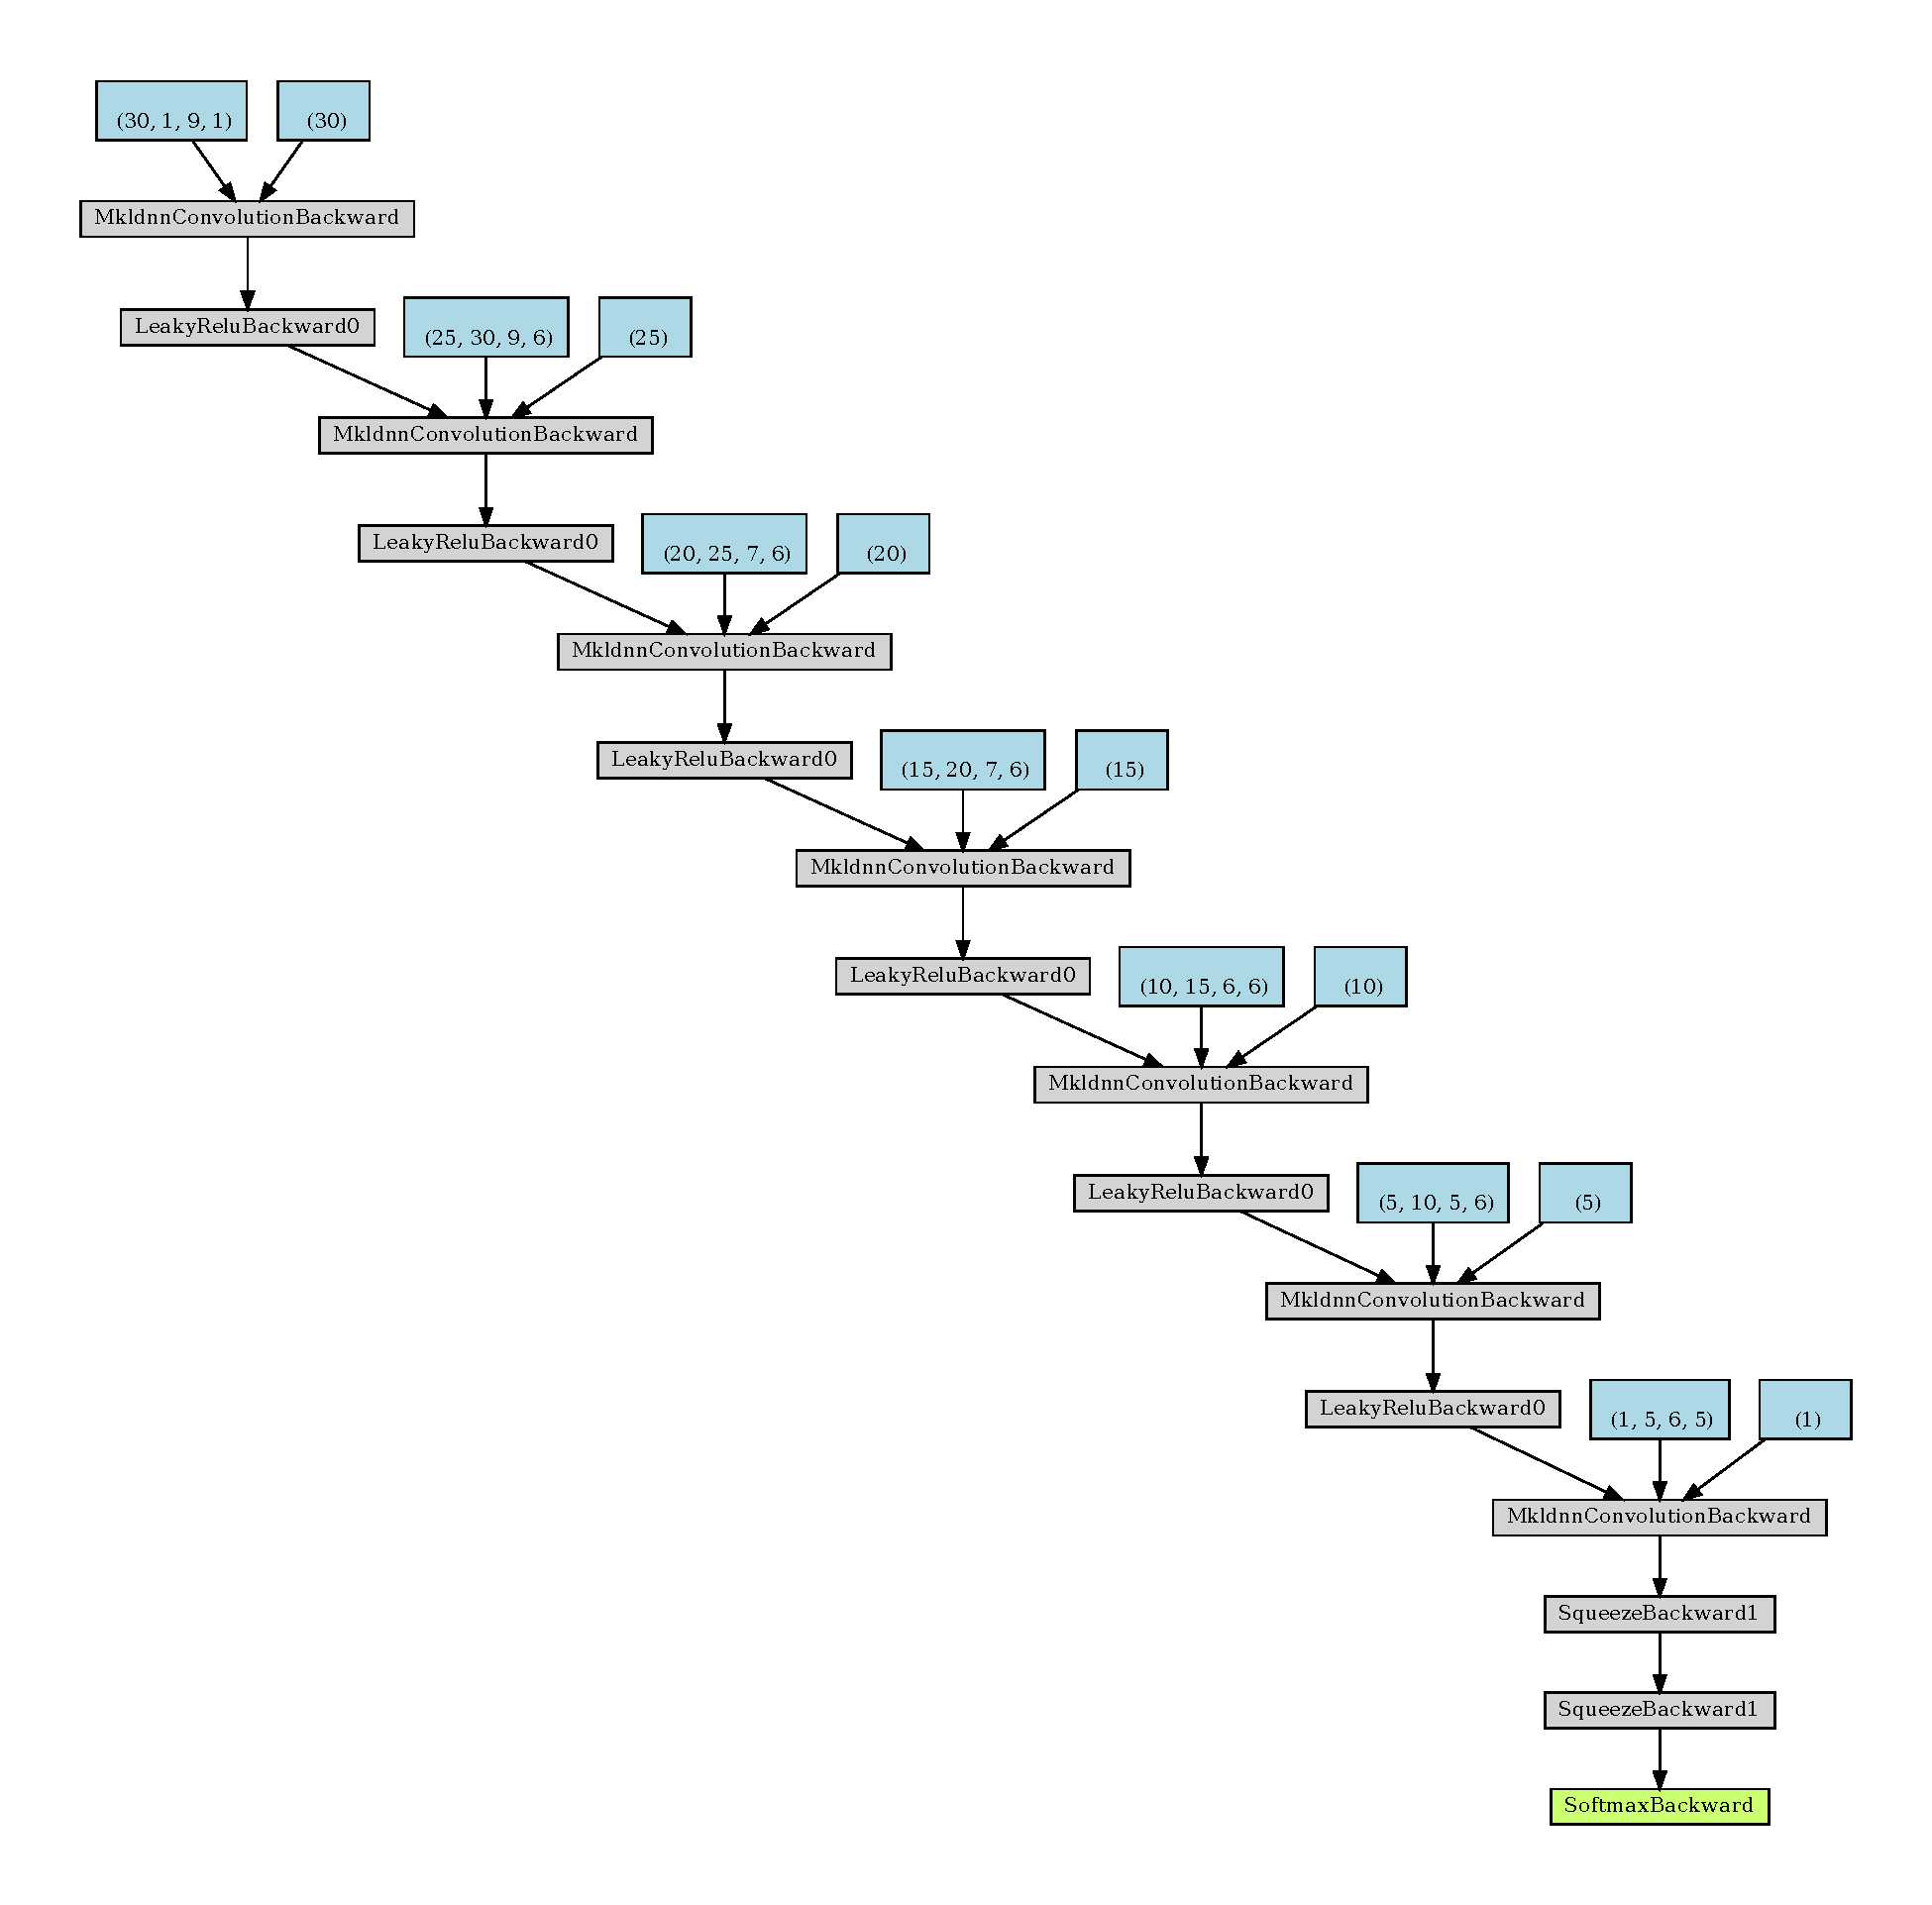
\includegraphics[width=1.0\linewidth]{net.pdf}
    \caption{CNN结构}
\end{figure}

我们使用了Jinping模拟数据的前4个:final-0.h5 - final-3.h5作为训练集(train set),
取训练集中的5\%作为测试集(test set),对每个训练集遍历12次,每4次训练后用测试集测试一次并保存模型,最后选取测试中loss最低的模型。
在我们的测试中,loss最低为$0.6007$。作为对比,完全随即猜测得到的鉴别结果的loss,理论值为$\ln{2}\approx0.6932$。

\section{算法检测结果}
对final-0.h5使用CNN处理可以给出粒子鉴别结果,使用NVIDIA GeForce GTX 1080Ti显卡进行处理,用时约4min。

将上述结果与final-0.h5中的真值进行对比,得到以下ROC曲线,其AUC $\approx0.757$:
\begin{figure}[H]
    \centering
    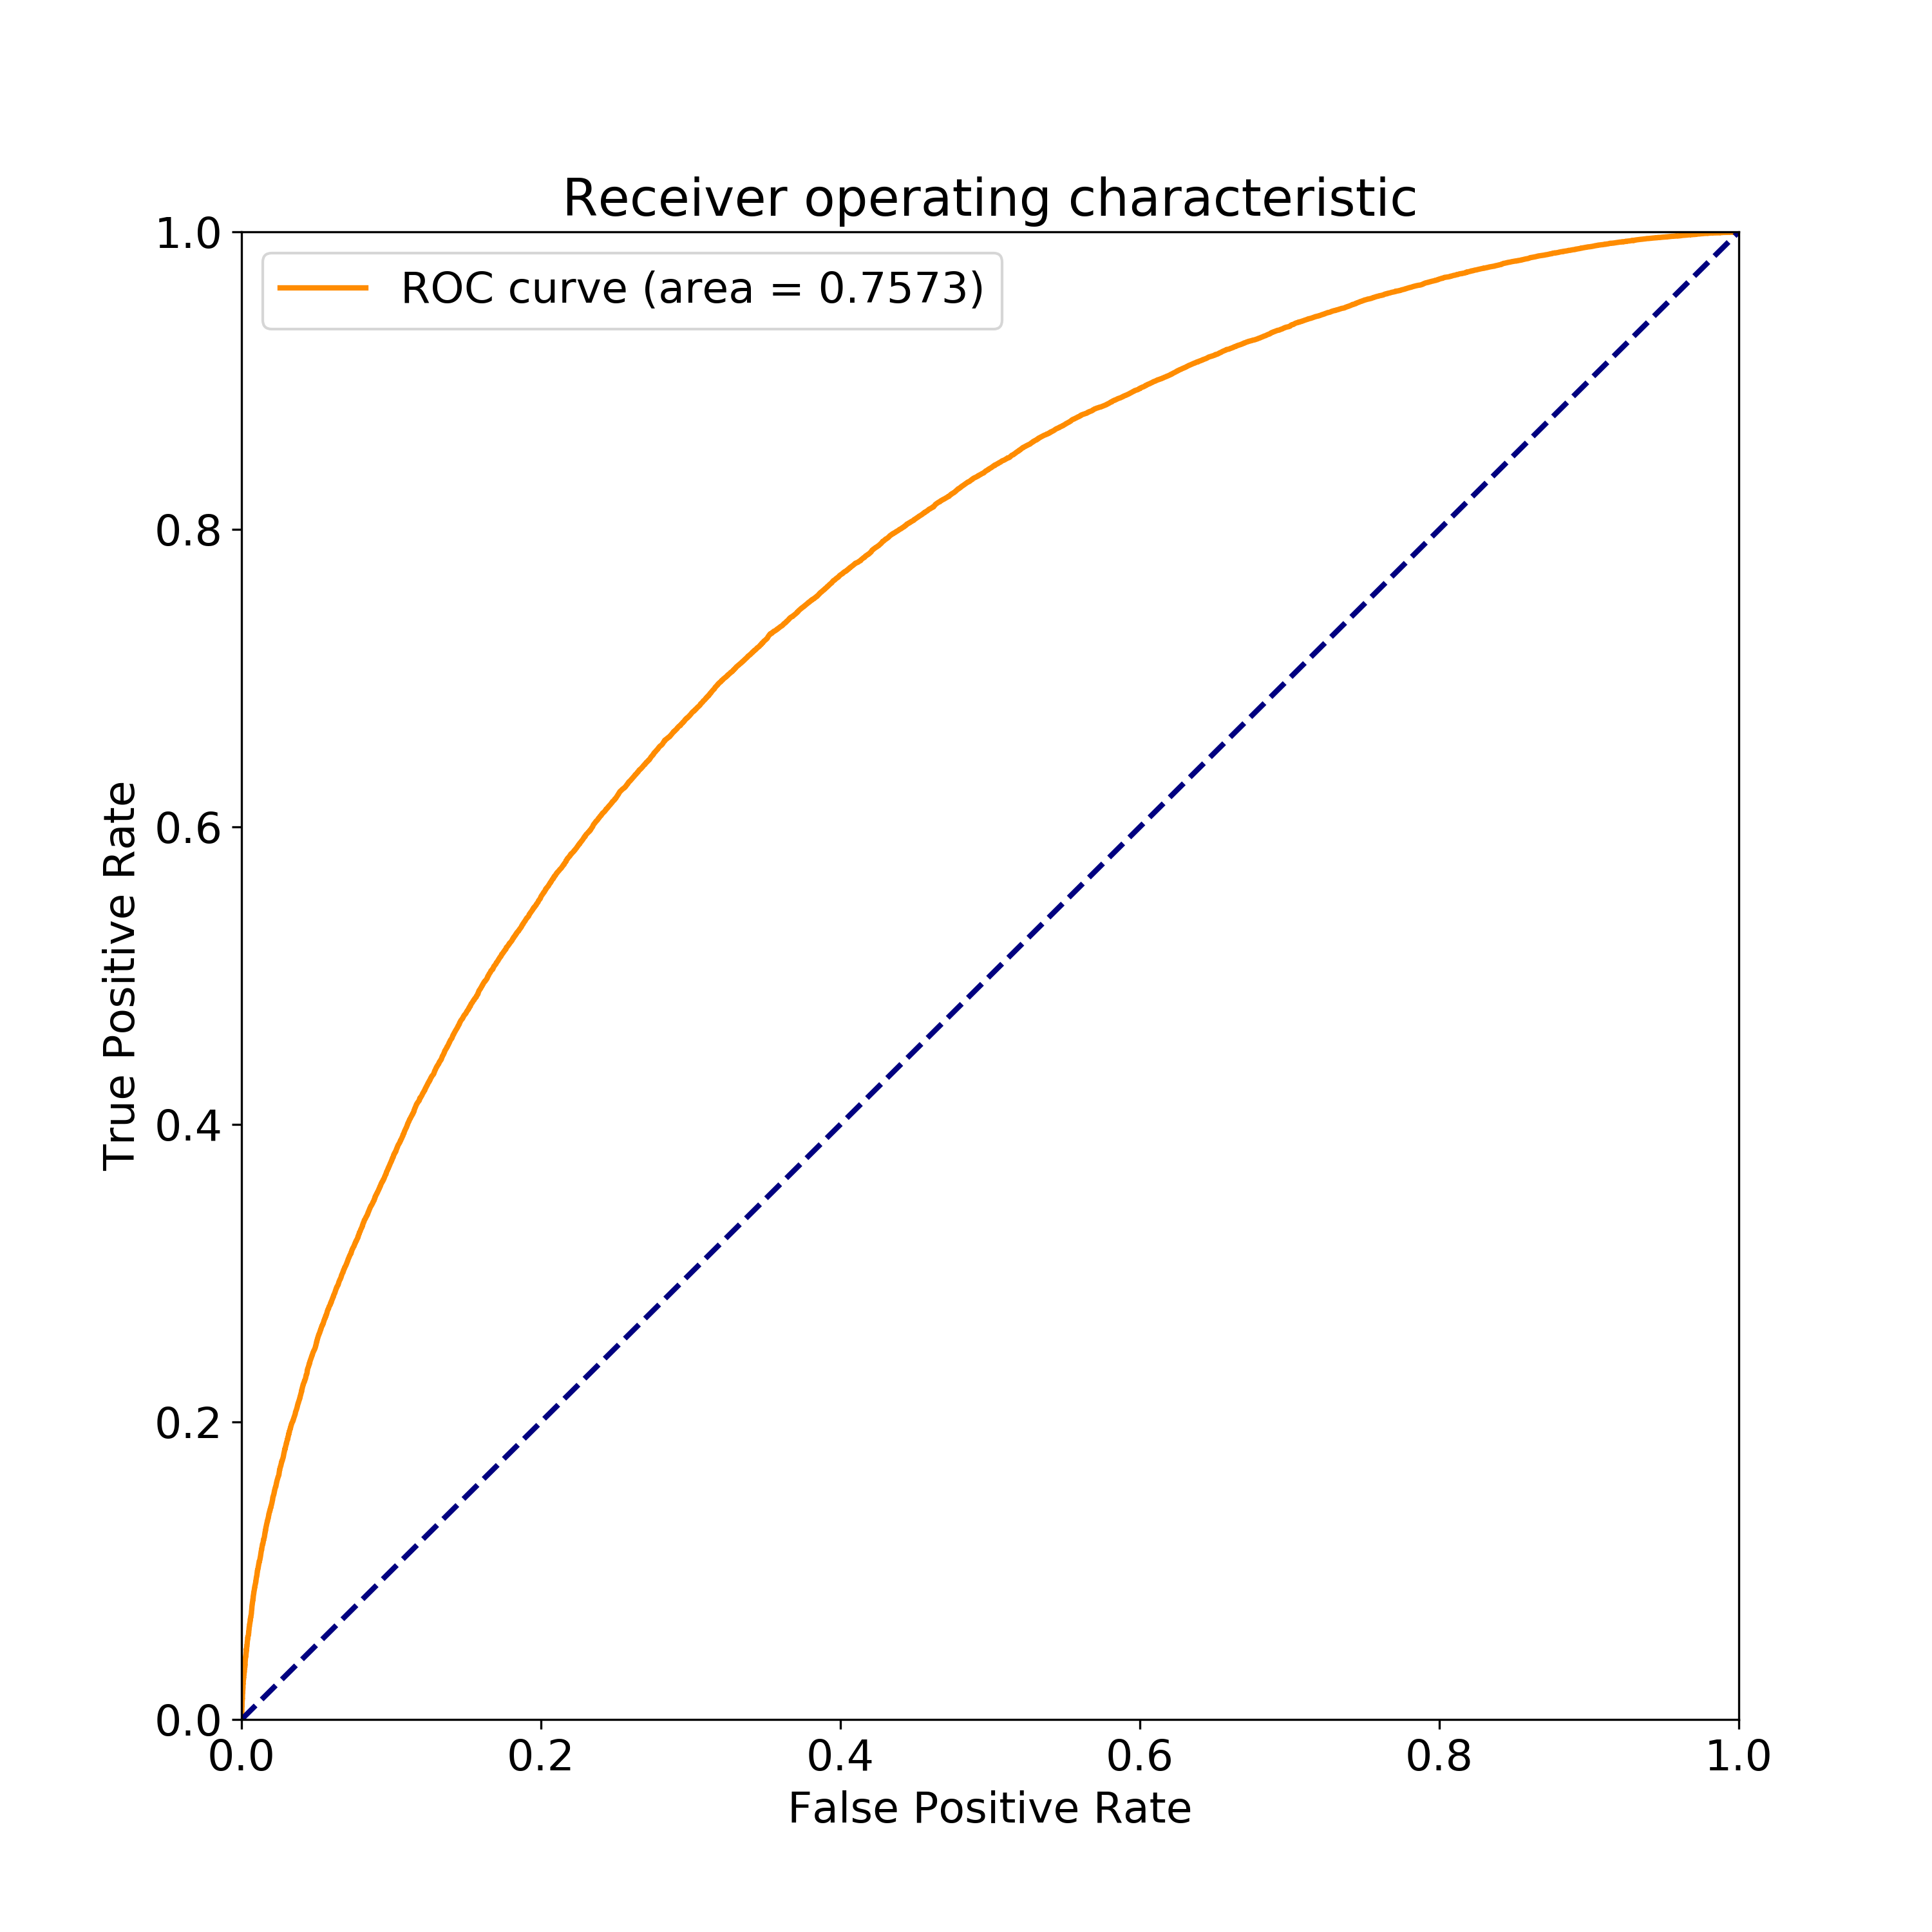
\includegraphics[width=1.0\linewidth]{ROC.png}
    \caption{CNN在final-0.h5上的ROC曲线}
\end{figure}

在Ghost Hunter2020决赛中,最终得到的AUC $\approx0.748$。

\section{改进}
\begin{itemize}
    \item 在制作训练集的过程中没有对PMT输出电压进行任何处理。在减去基线后,可能对CNN训练及预测结果有一定提升
    \item 激活函数LeakyReLU的参数选取中,只测试了$0.05$和$0.1$。可以通过交叉验证来优化激活函数。
\end{itemize}

\end{document}
